% !TeX root = main.tex

\chapter{Polygons}
\section{我们研究什么样的多边形}
\section{全等的严谨定义}
\section{二面体群和Cayley图}

% https://tex.stackexchange.com/questions/56442/what-are-some-good-examples-of-latex-cayley-diagrams

\usetikzlibrary{positioning}
\usetikzlibrary{petri}
\tikzset{state/.style={circle,draw=gray,inner
    sep=0pt,minimum size=7mm,label=center:$#1$,name=#1},
    redarrow/.style={->, red,
    fill=none,>=stealth},bluearrow/.style={->, blue,
    fill=none,>=stealth},
redline/.style={-,red,fill=none},blueline/.style={-,blue,fill=none}}

\begin{figure}[ht]
    \centering
    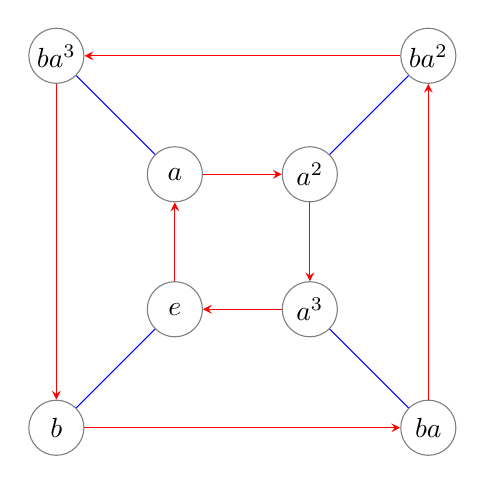
\begin{tikzpicture}
        \node[state=e]{};
        \node[state=a,above=of e]{};
        \node[state=a^2,right=of a]{};
        \node[state=a^3,below=of a^2]{};
        \node[state=b,below left=of e]{};
        \node[state=ba^3,above left=of a]{};
        \node[state=ba^2,above right=of a^2]{};
        \node[state=ba,below right=of a^3]{};
        \draw[redarrow](e)--(a);\draw[redarrow](b)--(ba);
        \draw[redarrow](a)--(a^2);\draw[redarrow](ba)--(ba^2);
        \draw[redarrow](a^2)--(a^3);\draw[redarrow](ba^2)--(ba^3);
        \draw[redarrow](a^3)--(e);\draw[redarrow](ba^3)--(b);
        \draw[blueline](e)--(b);
        \draw[blueline](a)--(ba^3);
        \draw[blueline](a^2)--(ba^2);
        \draw[blueline](a^3)--(ba);
    \end{tikzpicture}
\end{figure}
